\documentclass[1p]{elsarticle_modified}
%\bibliographystyle{elsarticle-num}

%\usepackage[colorlinks]{hyperref}
%\usepackage{abbrmath_seonhwa} %\Abb, \Ascr, \Acal ,\Abf, \Afrak
\usepackage{amsfonts}
\usepackage{amssymb}
\usepackage{amsmath}
\usepackage{amsthm}
\usepackage{scalefnt}
\usepackage{amsbsy}
\usepackage{kotex}
\usepackage{caption}
\usepackage{subfig}
\usepackage{color}
\usepackage{graphicx}
\usepackage{xcolor} %% white, black, red, green, blue, cyan, magenta, yellow
\usepackage{float}
\usepackage{setspace}
\usepackage{hyperref}

\usepackage{tikz}
\usetikzlibrary{arrows}

\usepackage{multirow}
\usepackage{array} % fixed length table
\usepackage{hhline}

%%%%%%%%%%%%%%%%%%%%%
\makeatletter
\renewcommand*\env@matrix[1][\arraystretch]{%
	\edef\arraystretch{#1}%
	\hskip -\arraycolsep
	\let\@ifnextchar\new@ifnextchar
	\array{*\c@MaxMatrixCols c}}
\makeatother %https://tex.stackexchange.com/questions/14071/how-can-i-increase-the-line-spacing-in-a-matrix
%%%%%%%%%%%%%%%

\usepackage[normalem]{ulem}

\newcommand{\msout}[1]{\ifmmode\text{\sout{\ensuremath{#1}}}\else\sout{#1}\fi}
%SOURCE: \msout is \stkout macro in https://tex.stackexchange.com/questions/20609/strikeout-in-math-mode

\newcommand{\cancel}[1]{
	\ifmmode
	{\color{red}\msout{#1}}
	\else
	{\color{red}\sout{#1}}
	\fi
}

\newcommand{\add}[1]{
	{\color{blue}\uwave{#1}}
}

\newcommand{\replace}[2]{
	\ifmmode
	{\color{red}\msout{#1}}{\color{blue}\uwave{#2}}
	\else
	{\color{red}\sout{#1}}{\color{blue}\uwave{#2}}
	\fi
}

\newcommand{\Sol}{\mathcal{S}} %segment
\newcommand{\D}{D} %diagram
\newcommand{\A}{\mathcal{A}} %arc


%%%%%%%%%%%%%%%%%%%%%%%%%%%%%5 test

\def\sl{\operatorname{\textup{SL}}(2,\Cbb)}
\def\psl{\operatorname{\textup{PSL}}(2,\Cbb)}
\def\quan{\mkern 1mu \triangleright \mkern 1mu}

\theoremstyle{definition}
\newtheorem{thm}{Theorem}[section]
\newtheorem{prop}[thm]{Proposition}
\newtheorem{lem}[thm]{Lemma}
\newtheorem{ques}[thm]{Question}
\newtheorem{cor}[thm]{Corollary}
\newtheorem{defn}[thm]{Definition}
\newtheorem{exam}[thm]{Example}
\newtheorem{rmk}[thm]{Remark}
\newtheorem{alg}[thm]{Algorithm}

\newcommand{\I}{\sqrt{-1}}
\begin{document}

%\begin{frontmatter}
%
%\title{Boundary parabolic representations of knots up to 8 crossings}
%
%%% Group authors per affiliation:
%\author{Yunhi Cho} 
%\address{Department of Mathematics, University of Seoul, Seoul, Korea}
%\ead{yhcho@uos.ac.kr}
%
%
%\author{Seonhwa Kim} %\fnref{s_kim}}
%\address{Center for Geometry and Physics, Institute for Basic Science, Pohang, 37673, Korea}
%\ead{ryeona17@ibs.re.kr}
%
%\author{Hyuk Kim}
%\address{Department of Mathematical Sciences, Seoul National University, Seoul 08826, Korea}
%\ead{hyukkim@snu.ac.kr}
%
%\author{Seokbeom Yoon}
%\address{Department of Mathematical Sciences, Seoul National University, Seoul, 08826,  Korea}
%\ead{sbyoon15@snu.ac.kr}
%
%\begin{abstract}
%We find all boundary parabolic representation of knots up to 8 crossings.
%
%\end{abstract}
%\begin{keyword}
%    \MSC[2010] 57M25 
%\end{keyword}
%
%\end{frontmatter}

%\linenumbers
%\tableofcontents
%
\newcommand\colored[1]{\textcolor{white}{\rule[-0.35ex]{0.8em}{1.4ex}}\kern-0.8em\color{red} #1}%
%\newcommand\colored[1]{\textcolor{white}{ #1}\kern-2.17ex	\textcolor{white}{ #1}\kern-1.81ex	\textcolor{white}{ #1}\kern-2.15ex\color{red}#1	}

{\Large $\underline{12n_{0176}~(K12n_{0176})}$}

\setlength{\tabcolsep}{10pt}
\renewcommand{\arraystretch}{1.6}
\vspace{1cm}\begin{tabular}{m{100pt}>{\centering\arraybackslash}m{274pt}}
\multirow{5}{120pt}{
	\centering
	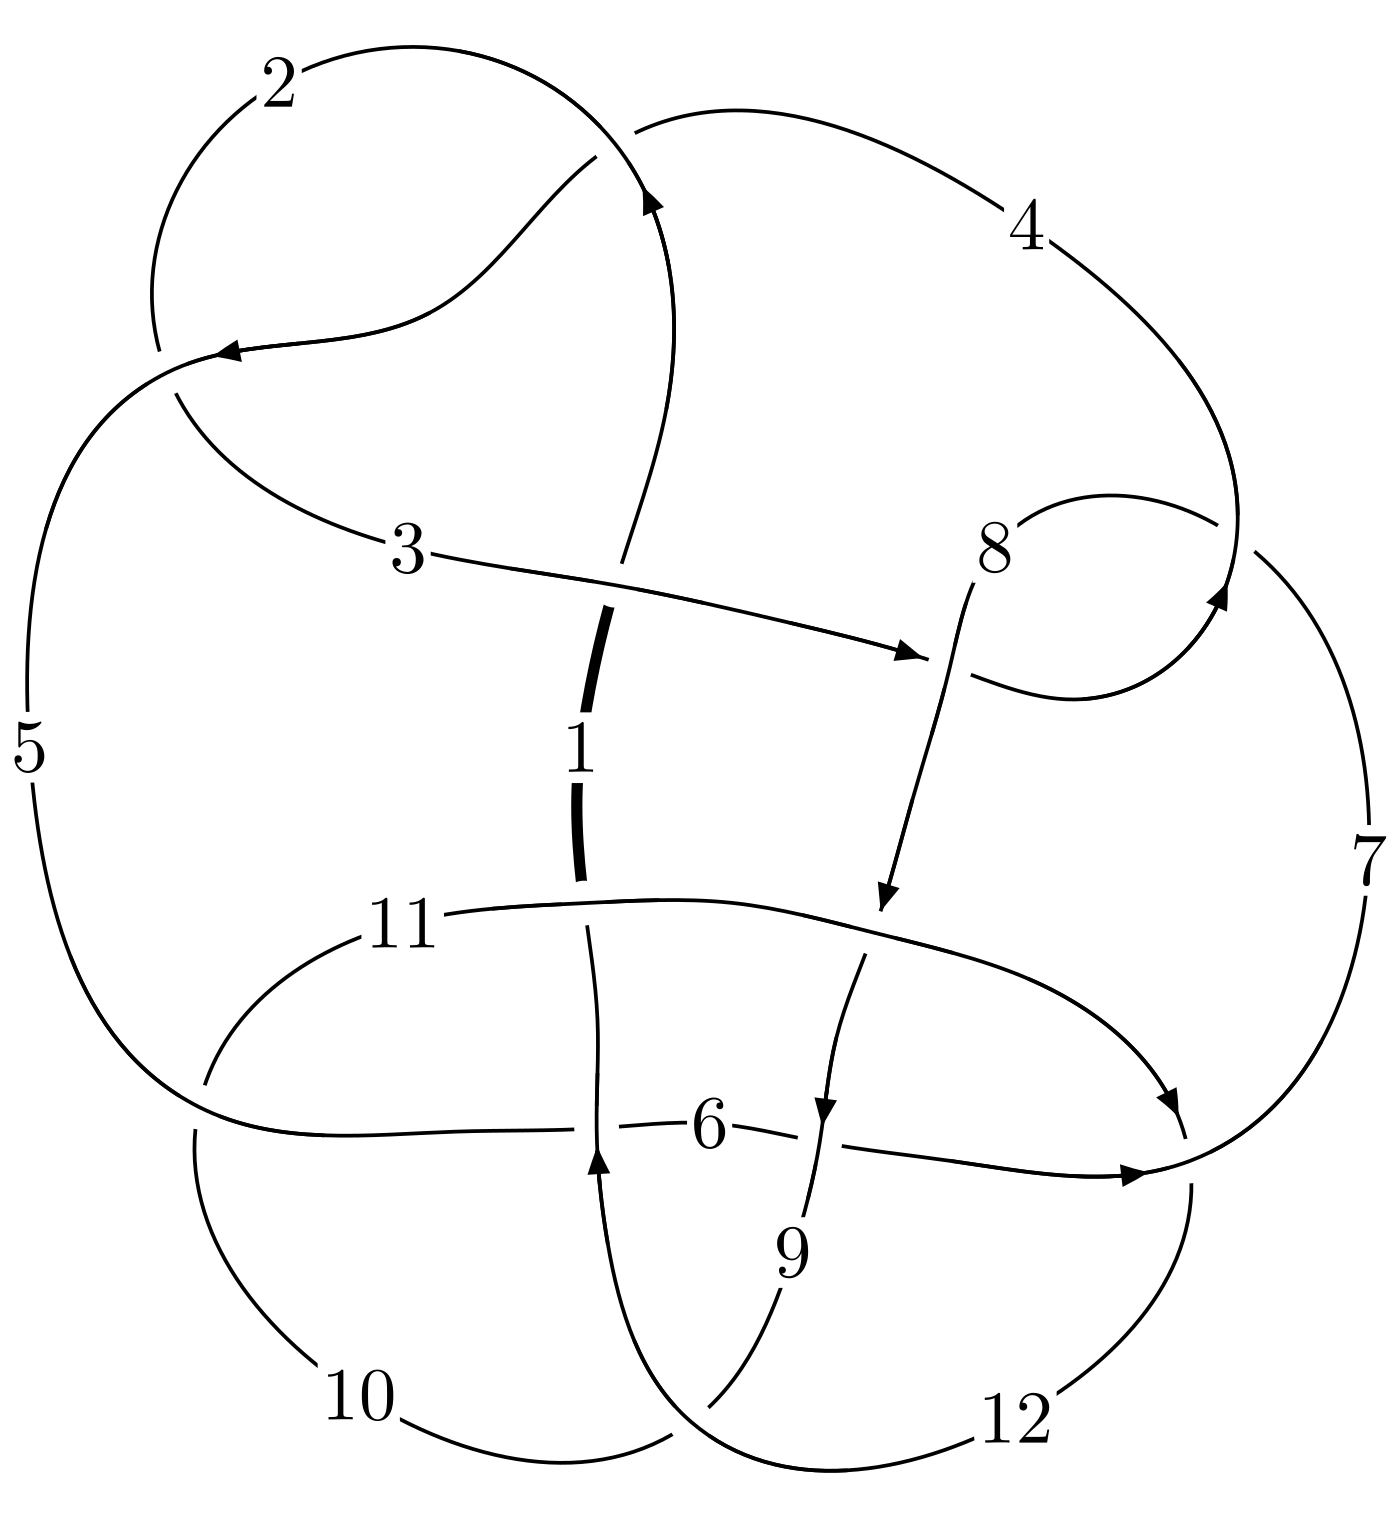
\includegraphics[width=112pt]{../../../GIT/diagram.site/Diagrams/png/2265_12n_0176.png}\\
\ \ \ A knot diagram\footnotemark}&
\allowdisplaybreaks
\textbf{Linearized knot diagam} \\
\cline{2-2}
 &
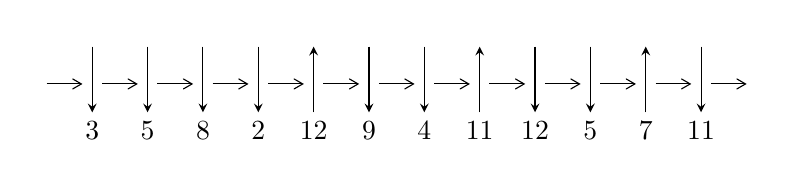
\begin{tikzpicture}[x=20pt, y=17pt]
	% nodes
	\node (C0) at (0, 0) {};
	\node (C1) at (1, 0) {};
	\node (C1U) at (1, +1) {};
	\node (C1D) at (1, -1) {3};

	\node (C2) at (2, 0) {};
	\node (C2U) at (2, +1) {};
	\node (C2D) at (2, -1) {5};

	\node (C3) at (3, 0) {};
	\node (C3U) at (3, +1) {};
	\node (C3D) at (3, -1) {8};

	\node (C4) at (4, 0) {};
	\node (C4U) at (4, +1) {};
	\node (C4D) at (4, -1) {2};

	\node (C5) at (5, 0) {};
	\node (C5U) at (5, +1) {};
	\node (C5D) at (5, -1) {12};

	\node (C6) at (6, 0) {};
	\node (C6U) at (6, +1) {};
	\node (C6D) at (6, -1) {9};

	\node (C7) at (7, 0) {};
	\node (C7U) at (7, +1) {};
	\node (C7D) at (7, -1) {4};

	\node (C8) at (8, 0) {};
	\node (C8U) at (8, +1) {};
	\node (C8D) at (8, -1) {11};

	\node (C9) at (9, 0) {};
	\node (C9U) at (9, +1) {};
	\node (C9D) at (9, -1) {12};

	\node (C10) at (10, 0) {};
	\node (C10U) at (10, +1) {};
	\node (C10D) at (10, -1) {5};

	\node (C11) at (11, 0) {};
	\node (C11U) at (11, +1) {};
	\node (C11D) at (11, -1) {7};

	\node (C12) at (12, 0) {};
	\node (C12U) at (12, +1) {};
	\node (C12D) at (12, -1) {11};
	\node (C13) at (13, 0) {};

	% arrows
	\draw[->,>={angle 60}]
	(C0) edge (C1) (C1) edge (C2) (C2) edge (C3) (C3) edge (C4) (C4) edge (C5) (C5) edge (C6) (C6) edge (C7) (C7) edge (C8) (C8) edge (C9) (C9) edge (C10) (C10) edge (C11) (C11) edge (C12) (C12) edge (C13) ;	\draw[->,>=stealth]
	(C1U) edge (C1D) (C2U) edge (C2D) (C3U) edge (C3D) (C4U) edge (C4D) (C5D) edge (C5U) (C6U) edge (C6D) (C7U) edge (C7D) (C8D) edge (C8U) (C9U) edge (C9D) (C10U) edge (C10D) (C11D) edge (C11U) (C12U) edge (C12D) ;
	\end{tikzpicture} \\
\hhline{~~} \\& 
\textbf{Solving Sequence} \\ \cline{2-2} 
 &
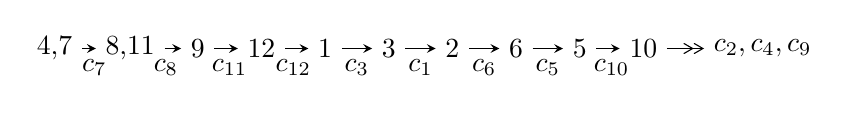
\begin{tikzpicture}[x=23pt, y=7pt]
	% node
	\node (A0) at (-1/8, 0) {4,7};
	\node (A1) at (17/16, 0) {8,11};
	\node (A2) at (17/8, 0) {9};
	\node (A3) at (25/8, 0) {12};
	\node (A4) at (33/8, 0) {1};
	\node (A5) at (41/8, 0) {3};
	\node (A6) at (49/8, 0) {2};
	\node (A7) at (57/8, 0) {6};
	\node (A8) at (65/8, 0) {5};
	\node (A9) at (73/8, 0) {10};
	\node (C1) at (1/2, -1) {$c_{7}$};
	\node (C2) at (13/8, -1) {$c_{8}$};
	\node (C3) at (21/8, -1) {$c_{11}$};
	\node (C4) at (29/8, -1) {$c_{12}$};
	\node (C5) at (37/8, -1) {$c_{3}$};
	\node (C6) at (45/8, -1) {$c_{1}$};
	\node (C7) at (53/8, -1) {$c_{6}$};
	\node (C8) at (61/8, -1) {$c_{5}$};
	\node (C9) at (69/8, -1) {$c_{10}$};
	\node (A10) at (11, 0) {$c_{2},c_{4},c_{9}$};

	% edge
	\draw[->,>=stealth]	
	(A0) edge (A1) (A1) edge (A2) (A2) edge (A3) (A3) edge (A4) (A4) edge (A5) (A5) edge (A6) (A6) edge (A7) (A7) edge (A8) (A8) edge (A9) ;
	\draw[->>,>={angle 60}]	
	(A9) edge (A10);
\end{tikzpicture} \\ 

\end{tabular} \\

\footnotetext{
The image of knot diagram is generated by the software ``\textbf{Draw programme}" developed by Andrew Bartholomew(\url{http://www.layer8.co.uk/maths/draw/index.htm\#Running-draw}), where we modified some parts for our purpose(\url{https://github.com/CATsTAILs/LinksPainter}).
}\phantom \\ \newline 
\centering \textbf{Ideals for irreducible components\footnotemark of $X_{\text{par}}$} 
 
\begin{align*}
I^u_{1}&=\langle 
3.05361\times10^{37} u^{37}-6.31699\times10^{37} u^{36}+\cdots+7.79069\times10^{38} b-1.45053\times10^{39},\\
\phantom{I^u_{1}}&\phantom{= \langle  }6.57951\times10^{37} u^{37}-1.30883\times10^{38} u^{36}+\cdots+7.79069\times10^{38} a+3.29567\times10^{39},\;u^{38}-2 u^{37}+\cdots-16 u+64\rangle \\
I^u_{2}&=\langle 
- u^{11}-2 u^9-2 u^7+u^3+b,\;- u^{11}+u^{10}-3 u^9+3 u^8-4 u^7+5 u^6-2 u^5+4 u^4+u^3+2 u^2+a+u+1,\\
\phantom{I^u_{2}}&\phantom{= \langle  }u^{12}+3 u^{10}+5 u^8+4 u^6+2 u^4+u^2+1\rangle \\
I^u_{3}&=\langle 
- a^2 u^2-4 a^2 u-2 a^2+b+4 u+2,\;-4 a^2 u^2+a^3-2 a^2 u+16 u^2 a-6 a^2+7 a u-8 u^2+27 a-3 u-15,\\
\phantom{I^u_{3}}&\phantom{= \langle  }u^3+u^2+2 u+1\rangle \\
\\
I^v_{1}&=\langle 
a,\;-2 v^3-3 v^2+4 b-8 v-3,\;2 v^4+v^3+5 v^2- v+1\rangle \\
\end{align*}
\raggedright * 4 irreducible components of $\dim_{\mathbb{C}}=0$, with total 63 representations.\\
\footnotetext{All coefficients of polynomials are rational numbers. But the coefficients are sometimes approximated in decimal forms when there is not enough margin.}
\newpage
\renewcommand{\arraystretch}{1}
\centering \section*{I. $I^u_{1}= \langle 3.05\times10^{37} u^{37}-6.32\times10^{37} u^{36}+\cdots+7.79\times10^{38} b-1.45\times10^{39},\;6.58\times10^{37} u^{37}-1.31\times10^{38} u^{36}+\cdots+7.79\times10^{38} a+3.30\times10^{39},\;u^{38}-2 u^{37}+\cdots-16 u+64 \rangle$}
\flushleft \textbf{(i) Arc colorings}\\
\begin{tabular}{m{7pt} m{180pt} m{7pt} m{180pt} }
\flushright $a_{4}=$&$\begin{pmatrix}0\\u\end{pmatrix}$ \\
\flushright $a_{7}=$&$\begin{pmatrix}1\\0\end{pmatrix}$ \\
\flushright $a_{8}=$&$\begin{pmatrix}1\\u^2\end{pmatrix}$ \\
\flushright $a_{11}=$&$\begin{pmatrix}-0.0844535 u^{37}+0.168000 u^{36}+\cdots-5.59244 u-4.23026\\-0.0391956 u^{37}+0.0810838 u^{36}+\cdots-11.2341 u+1.86188\end{pmatrix}$ \\
\flushright $a_{9}=$&$\begin{pmatrix}-0.0835952 u^{37}+0.174732 u^{36}+\cdots-10.9131 u+0.727986\\0.0870239 u^{37}-0.136889 u^{36}+\cdots+10.6763 u+8.29286\end{pmatrix}$ \\
\flushright $a_{12}=$&$\begin{pmatrix}-0.123649 u^{37}+0.249084 u^{36}+\cdots-16.8266 u-2.36838\\-0.0391956 u^{37}+0.0810838 u^{36}+\cdots-11.2341 u+1.86188\end{pmatrix}$ \\
\flushright $a_{1}=$&$\begin{pmatrix}-0.100768 u^{37}+0.165433 u^{36}+\cdots-8.51486 u-7.59481\\-0.0261741 u^{37}+0.0152352 u^{36}+\cdots-1.41664 u-8.18193\end{pmatrix}$ \\
\flushright $a_{3}=$&$\begin{pmatrix}u\\u^3+u\end{pmatrix}$ \\
\flushright $a_{2}=$&$\begin{pmatrix}-0.0775401 u^{37}+0.125316 u^{36}+\cdots-7.03756 u-7.83004\\-0.0160423 u^{37}-0.00551256 u^{36}+\cdots-1.32448 u-8.82286\end{pmatrix}$ \\
\flushright $a_{6}=$&$\begin{pmatrix}-0.199765 u^{37}+0.392882 u^{36}+\cdots-29.9030 u-7.71626\\-0.0575627 u^{37}+0.156935 u^{36}+\cdots-18.3766 u+7.51449\end{pmatrix}$ \\
\flushright $a_{5}=$&$\begin{pmatrix}-0.0221640 u^{37}+0.0480035 u^{36}+\cdots-1.22673 u+2.89771\\0.0786038 u^{37}-0.117429 u^{36}+\cdots+7.28813 u+10.4925\end{pmatrix}$ \\
\flushright $a_{10}=$&$\begin{pmatrix}0.0238166 u^{37}-0.105781 u^{36}+\cdots+18.0697 u-10.6973\\0.0874152 u^{37}-0.224299 u^{36}+\cdots+22.3080 u-6.95902\end{pmatrix}$\\&\end{tabular}
\flushleft \textbf{(ii) Obstruction class $= -1$}\\~\\
\flushleft \textbf{(iii) Cusp Shapes $= -0.284536 u^{37}+0.695784 u^{36}+\cdots-86.8413 u+36.9834$}\\~\\
\newpage\renewcommand{\arraystretch}{1}
\flushleft \textbf{(iv) u-Polynomials at the component}\newline \\
\begin{tabular}{m{50pt}|m{274pt}}
Crossings & \hspace{64pt}u-Polynomials at each crossing \\
\hline $$\begin{aligned}c_{1}\end{aligned}$$&$\begin{aligned}
&u^{38}+16 u^{37}+\cdots+49 u+16
\end{aligned}$\\
\hline $$\begin{aligned}c_{2},c_{4}\end{aligned}$$&$\begin{aligned}
&u^{38}-4 u^{37}+\cdots-35 u+4
\end{aligned}$\\
\hline $$\begin{aligned}c_{3},c_{7}\end{aligned}$$&$\begin{aligned}
&u^{38}-2 u^{37}+\cdots-16 u+64
\end{aligned}$\\
\hline $$\begin{aligned}c_{5}\end{aligned}$$&$\begin{aligned}
&u^{38}+4 u^{37}+\cdots-28 u+49
\end{aligned}$\\
\hline $$\begin{aligned}c_{6},c_{10}\end{aligned}$$&$\begin{aligned}
&u^{38}-2 u^{37}+\cdots+42 u+9
\end{aligned}$\\
\hline $$\begin{aligned}c_{8}\end{aligned}$$&$\begin{aligned}
&u^{38}+14 u^{37}+\cdots+95422 u+43691
\end{aligned}$\\
\hline $$\begin{aligned}c_{9}\end{aligned}$$&$\begin{aligned}
&u^{38}-8 u^{37}+\cdots+235720 u+204268
\end{aligned}$\\
\hline $$\begin{aligned}c_{11}\end{aligned}$$&$\begin{aligned}
&u^{38}-2 u^{37}+\cdots+18 u+9
\end{aligned}$\\
\hline $$\begin{aligned}c_{12}\end{aligned}$$&$\begin{aligned}
&u^{38}+2 u^{37}+\cdots-576 u+81
\end{aligned}$\\
\hline
\end{tabular}\\~\\
\newpage\renewcommand{\arraystretch}{1}
\flushleft \textbf{(v) Riley Polynomials at the component}\newline \\
\begin{tabular}{m{50pt}|m{274pt}}
Crossings & \hspace{64pt}Riley Polynomials at each crossing \\
\hline $$\begin{aligned}c_{1}\end{aligned}$$&$\begin{aligned}
&y^{38}+16 y^{37}+\cdots+137023 y+256
\end{aligned}$\\
\hline $$\begin{aligned}c_{2},c_{4}\end{aligned}$$&$\begin{aligned}
&y^{38}-16 y^{37}+\cdots-49 y+16
\end{aligned}$\\
\hline $$\begin{aligned}c_{3},c_{7}\end{aligned}$$&$\begin{aligned}
&y^{38}+24 y^{37}+\cdots+78592 y+4096
\end{aligned}$\\
\hline $$\begin{aligned}c_{5}\end{aligned}$$&$\begin{aligned}
&y^{38}-92 y^{37}+\cdots-3136 y+2401
\end{aligned}$\\
\hline $$\begin{aligned}c_{6},c_{10}\end{aligned}$$&$\begin{aligned}
&y^{38}+58 y^{37}+\cdots+2304 y+81
\end{aligned}$\\
\hline $$\begin{aligned}c_{8}\end{aligned}$$&$\begin{aligned}
&y^{38}-48 y^{37}+\cdots-15294799908 y+1908903481
\end{aligned}$\\
\hline $$\begin{aligned}c_{9}\end{aligned}$$&$\begin{aligned}
&y^{38}+70 y^{37}+\cdots+426020361080 y+41725415824
\end{aligned}$\\
\hline $$\begin{aligned}c_{11}\end{aligned}$$&$\begin{aligned}
&y^{38}+2 y^{37}+\cdots-576 y+81
\end{aligned}$\\
\hline $$\begin{aligned}c_{12}\end{aligned}$$&$\begin{aligned}
&y^{38}+82 y^{37}+\cdots+166536 y+6561
\end{aligned}$\\
\hline
\end{tabular}\\~\\
\newpage\flushleft \textbf{(vi) Complex Volumes and Cusp Shapes}
$$\begin{array}{c|c|c}  
\text{Solutions to }I^u_{1}& \I (\text{vol} + \sqrt{-1}CS) & \text{Cusp shape}\\
 \hline 
\begin{aligned}
u &= \phantom{-}0.988171 + 0.101317 I \\
a &= \phantom{-}0.357719 + 0.096343 I \\
b &= -0.706300 - 0.532125 I\end{aligned}
 & \phantom{-}0.60571 + 3.27765 I & -3.71492 - 6.11137 I \\ \hline\begin{aligned}
u &= \phantom{-}0.988171 - 0.101317 I \\
a &= \phantom{-}0.357719 - 0.096343 I \\
b &= -0.706300 + 0.532125 I\end{aligned}
 & \phantom{-}0.60571 - 3.27765 I & -3.71492 + 6.11137 I \\ \hline\begin{aligned}
u &= -0.859103 + 0.407305 I \\
a &= \phantom{-}0.195881 + 0.507732 I \\
b &= -0.415895 - 0.161770 I\end{aligned}
 & -0.113764 - 0.661154 I & -3.22428 + 0.50932 I \\ \hline\begin{aligned}
u &= -0.859103 - 0.407305 I \\
a &= \phantom{-}0.195881 - 0.507732 I \\
b &= -0.415895 + 0.161770 I\end{aligned}
 & -0.113764 + 0.661154 I & -3.22428 - 0.50932 I \\ \hline\begin{aligned}
u &= -0.057356 + 0.905930 I \\
a &= \phantom{-}0.690281 - 0.347775 I \\
b &= -0.294609 - 0.999645 I\end{aligned}
 & -0.317569 + 1.038530 I & -6.65259 - 1.29718 I \\ \hline\begin{aligned}
u &= -0.057356 - 0.905930 I \\
a &= \phantom{-}0.690281 + 0.347775 I \\
b &= -0.294609 + 0.999645 I\end{aligned}
 & -0.317569 - 1.038530 I & -6.65259 + 1.29718 I \\ \hline\begin{aligned}
u &= \phantom{-}0.513402 + 1.056580 I \\
a &= -0.548129 - 0.950989 I \\
b &= \phantom{-}0.629901 - 0.115553 I\end{aligned}
 & \phantom{-}4.15976 - 1.13418 I & \phantom{-}1.31812 + 0.91951 I \\ \hline\begin{aligned}
u &= \phantom{-}0.513402 - 1.056580 I \\
a &= -0.548129 + 0.950989 I \\
b &= \phantom{-}0.629901 + 0.115553 I\end{aligned}
 & \phantom{-}4.15976 + 1.13418 I & \phantom{-}1.31812 - 0.91951 I \\ \hline\begin{aligned}
u &= \phantom{-}0.499541 + 1.066880 I \\
a &= \phantom{-}0.678051 + 0.671685 I \\
b &= -0.123848 + 1.082220 I\end{aligned}
 & -1.77296 - 5.49964 I & -11.19640 + 5.85708 I \\ \hline\begin{aligned}
u &= \phantom{-}0.499541 - 1.066880 I \\
a &= \phantom{-}0.678051 - 0.671685 I \\
b &= -0.123848 - 1.082220 I\end{aligned}
 & -1.77296 + 5.49964 I & -11.19640 - 5.85708 I\\
 \hline 
 \end{array}$$\newpage$$\begin{array}{c|c|c}  
\text{Solutions to }I^u_{1}& \I (\text{vol} + \sqrt{-1}CS) & \text{Cusp shape}\\
 \hline 
\begin{aligned}
u &= \phantom{-}0.636697 + 0.515733 I \\
a &= \phantom{-}1.48373 + 1.08936 I \\
b &= \phantom{-}0.050362 + 0.915692 I\end{aligned}
 & -3.49167 + 1.02692 I & -15.5440 - 0.4261 I \\ \hline\begin{aligned}
u &= \phantom{-}0.636697 - 0.515733 I \\
a &= \phantom{-}1.48373 - 1.08936 I \\
b &= \phantom{-}0.050362 - 0.915692 I\end{aligned}
 & -3.49167 - 1.02692 I & -15.5440 + 0.4261 I \\ \hline\begin{aligned}
u &= -0.632708 + 1.049740 I \\
a &= -0.318350 + 0.929181 I \\
b &= \phantom{-}0.386295 + 0.336655 I\end{aligned}
 & \phantom{-}1.72214 + 6.04516 I & -1.25225 - 6.03705 I \\ \hline\begin{aligned}
u &= -0.632708 - 1.049740 I \\
a &= -0.318350 - 0.929181 I \\
b &= \phantom{-}0.386295 - 0.336655 I\end{aligned}
 & \phantom{-}1.72214 - 6.04516 I & -1.25225 + 6.03705 I \\ \hline\begin{aligned}
u &= -0.116308 + 0.741636 I \\
a &= -1.59041 + 2.36341 I \\
b &= \phantom{-}0.483477 - 0.463055 I\end{aligned}
 & -1.04131 - 1.37519 I & -0.70276 + 2.28236 I \\ \hline\begin{aligned}
u &= -0.116308 - 0.741636 I \\
a &= -1.59041 - 2.36341 I \\
b &= \phantom{-}0.483477 + 0.463055 I\end{aligned}
 & -1.04131 + 1.37519 I & -0.70276 - 2.28236 I \\ \hline\begin{aligned}
u &= -0.120470 + 1.245000 I \\
a &= \phantom{-}1.85282 + 0.54192 I \\
b &= -1.07360 - 1.05803 I\end{aligned}
 & \phantom{-}8.23228 + 3.92903 I & -3.32062 - 2.35045 I \\ \hline\begin{aligned}
u &= -0.120470 - 1.245000 I \\
a &= \phantom{-}1.85282 - 0.54192 I \\
b &= -1.07360 + 1.05803 I\end{aligned}
 & \phantom{-}8.23228 - 3.92903 I & -3.32062 + 2.35045 I \\ \hline\begin{aligned}
u &= \phantom{-}1.330860 + 0.099817 I \\
a &= -0.271191 - 0.510477 I \\
b &= \phantom{-}1.14380 - 1.00359 I\end{aligned}
 & \phantom{-}10.21150 - 1.13879 I & -3.05135 - 0.25663 I \\ \hline\begin{aligned}
u &= \phantom{-}1.330860 - 0.099817 I \\
a &= -0.271191 + 0.510477 I \\
b &= \phantom{-}1.14380 + 1.00359 I\end{aligned}
 & \phantom{-}10.21150 + 1.13879 I & -3.05135 + 0.25663 I\\
 \hline 
 \end{array}$$\newpage$$\begin{array}{c|c|c}  
\text{Solutions to }I^u_{1}& \I (\text{vol} + \sqrt{-1}CS) & \text{Cusp shape}\\
 \hline 
\begin{aligned}
u &= -1.316680 + 0.320236 I \\
a &= -0.223799 - 0.516251 I \\
b &= \phantom{-}1.05336 - 1.13298 I\end{aligned}
 & \phantom{-}9.76921 - 6.87392 I & -3.78751 + 4.34762 I \\ \hline\begin{aligned}
u &= -1.316680 - 0.320236 I \\
a &= -0.223799 + 0.516251 I \\
b &= \phantom{-}1.05336 + 1.13298 I\end{aligned}
 & \phantom{-}9.76921 + 6.87392 I & -3.78751 - 4.34762 I \\ \hline\begin{aligned}
u &= -0.20211 + 1.41718 I \\
a &= -1.355950 - 0.243842 I \\
b &= \phantom{-}0.995463 + 0.570318 I\end{aligned}
 & \phantom{-}6.08307 + 2.78224 I & \phantom{-0.000000 } 0. - 2.28655 I \\ \hline\begin{aligned}
u &= -0.20211 - 1.41718 I \\
a &= -1.355950 + 0.243842 I \\
b &= \phantom{-}0.995463 - 0.570318 I\end{aligned}
 & \phantom{-}6.08307 - 2.78224 I & \phantom{-0.000000 -}0. + 2.28655 I \\ \hline\begin{aligned}
u &= -0.072001 + 0.547844 I \\
a &= -0.238648 - 0.632863 I \\
b &= \phantom{-}0.790221 - 0.913835 I\end{aligned}
 & \phantom{-}5.57535 - 2.98438 I & \phantom{-}5.83310 - 0.97501 I \\ \hline\begin{aligned}
u &= -0.072001 - 0.547844 I \\
a &= -0.238648 + 0.632863 I \\
b &= \phantom{-}0.790221 + 0.913835 I\end{aligned}
 & \phantom{-}5.57535 + 2.98438 I & \phantom{-}5.83310 + 0.97501 I \\ \hline\begin{aligned}
u &= \phantom{-}0.52721 + 1.38450 I \\
a &= -1.43906 - 0.13679 I \\
b &= \phantom{-}0.974228 - 0.765508 I\end{aligned}
 & \phantom{-}4.71055 - 8.92356 I & -6.00000 + 7.15584 I \\ \hline\begin{aligned}
u &= \phantom{-}0.52721 - 1.38450 I \\
a &= -1.43906 + 0.13679 I \\
b &= \phantom{-}0.974228 + 0.765508 I\end{aligned}
 & \phantom{-}4.71055 + 8.92356 I & -6.00000 - 7.15584 I \\ \hline\begin{aligned}
u &= -0.194741 + 0.457992 I \\
a &= \phantom{-}0.933635 - 0.070105 I \\
b &= -0.245714 - 0.786744 I\end{aligned}
 & -0.451389 + 1.231000 I & -5.01122 - 5.21291 I \\ \hline\begin{aligned}
u &= -0.194741 - 0.457992 I \\
a &= \phantom{-}0.933635 + 0.070105 I \\
b &= -0.245714 + 0.786744 I\end{aligned}
 & -0.451389 - 1.231000 I & -5.01122 + 5.21291 I\\
 \hline 
 \end{array}$$\newpage$$\begin{array}{c|c|c}  
\text{Solutions to }I^u_{1}& \I (\text{vol} + \sqrt{-1}CS) & \text{Cusp shape}\\
 \hline 
\begin{aligned}
u &= -0.74805 + 1.38740 I \\
a &= \phantom{-}1.46219 - 0.60021 I \\
b &= -0.96971 - 1.27489 I\end{aligned}
 & \phantom{-}13.1525 + 14.1820 I & \phantom{-0.000000 } 0 \\ \hline\begin{aligned}
u &= -0.74805 - 1.38740 I \\
a &= \phantom{-}1.46219 + 0.60021 I \\
b &= -0.96971 + 1.27489 I\end{aligned}
 & \phantom{-}13.1525 - 14.1820 I & \phantom{-0.000000 } 0 \\ \hline\begin{aligned}
u &= \phantom{-}0.53207 + 1.50578 I \\
a &= \phantom{-}1.45703 + 0.26277 I \\
b &= -1.06014 + 1.24087 I\end{aligned}
 & \phantom{-}15.4688 - 7.6978 I & \phantom{-0.000000 } 0 \\ \hline\begin{aligned}
u &= \phantom{-}0.53207 - 1.50578 I \\
a &= \phantom{-}1.45703 - 0.26277 I \\
b &= -1.06014 - 1.24087 I\end{aligned}
 & \phantom{-}15.4688 + 7.6978 I & \phantom{-0.000000 } 0 \\ \hline\begin{aligned}
u &= \phantom{-}0.64254 + 1.50454 I \\
a &= \phantom{-}0.570332 + 0.670108 I \\
b &= -1.32203 - 0.83464 I\end{aligned}
 & \phantom{-}14.6938 - 5.9617 I & \phantom{-0.000000 } 0 \\ \hline\begin{aligned}
u &= \phantom{-}0.64254 - 1.50454 I \\
a &= \phantom{-}0.570332 - 0.670108 I \\
b &= -1.32203 + 0.83464 I\end{aligned}
 & \phantom{-}14.6938 + 5.9617 I & \phantom{-0.000000 } 0 \\ \hline\begin{aligned}
u &= -0.35097 + 1.60847 I \\
a &= \phantom{-}0.866365 - 0.578189 I \\
b &= -1.29525 + 0.97186 I\end{aligned}
 & \phantom{-}16.4349 - 0.8014 I & \phantom{-0.000000 } 0 \\ \hline\begin{aligned}
u &= -0.35097 - 1.60847 I \\
a &= \phantom{-}0.866365 + 0.578189 I \\
b &= -1.29525 - 0.97186 I\end{aligned}
 & \phantom{-}16.4349 + 0.8014 I & \phantom{-0.000000 } 0\\
 \hline 
 \end{array}$$\newpage\newpage\renewcommand{\arraystretch}{1}
\centering \section*{II. $I^u_{2}= \langle - u^{11}-2 u^9-2 u^7+u^3+b,\;- u^{11}+u^{10}+\cdots+a+1,\;u^{12}+3 u^{10}+5 u^8+4 u^6+2 u^4+u^2+1 \rangle$}
\flushleft \textbf{(i) Arc colorings}\\
\begin{tabular}{m{7pt} m{180pt} m{7pt} m{180pt} }
\flushright $a_{4}=$&$\begin{pmatrix}0\\u\end{pmatrix}$ \\
\flushright $a_{7}=$&$\begin{pmatrix}1\\0\end{pmatrix}$ \\
\flushright $a_{8}=$&$\begin{pmatrix}1\\u^2\end{pmatrix}$ \\
\flushright $a_{11}=$&$\begin{pmatrix}u^{11}- u^{10}+3 u^9-3 u^8+4 u^7-5 u^6+2 u^5-4 u^4- u^3-2 u^2- u-1\\u^{11}+2 u^9+2 u^7- u^3\end{pmatrix}$ \\
\flushright $a_{9}=$&$\begin{pmatrix}2 u^{11}- u^{10}+5 u^9-3 u^8+6 u^7-5 u^6+2 u^5-4 u^4-2 u^3-3 u^2- u-1\\u^{11}+2 u^9+2 u^7- u^3\end{pmatrix}$ \\
\flushright $a_{12}=$&$\begin{pmatrix}2 u^{11}- u^{10}+5 u^9-3 u^8+6 u^7-5 u^6+2 u^5-4 u^4-2 u^3-2 u^2- u-1\\u^{11}+2 u^9+2 u^7- u^3\end{pmatrix}$ \\
\flushright $a_{1}=$&$\begin{pmatrix}u^{11}+2 u^9+2 u^7- u^3\\0\end{pmatrix}$ \\
\flushright $a_{3}=$&$\begin{pmatrix}u\\u^3+u\end{pmatrix}$ \\
\flushright $a_{2}=$&$\begin{pmatrix}- u^7-2 u^5-2 u^3\\- u^7- u^5+u\end{pmatrix}$ \\
\flushright $a_{6}=$&$\begin{pmatrix}- u^{11}- u^{10}-4 u^9-3 u^8-6 u^7-5 u^6-5 u^5-4 u^4- u^3-2 u^2+2\\1\end{pmatrix}$ \\
\flushright $a_{5}=$&$\begin{pmatrix}u^9+2 u^7+3 u^5+2 u^3+u\\u^{11}+3 u^9+4 u^7+3 u^5+u^3+u\end{pmatrix}$ \\
\flushright $a_{10}=$&$\begin{pmatrix}u^{11}- u^{10}+3 u^9-3 u^8+4 u^7-5 u^6+2 u^5-4 u^4- u^3- u^2- u\\u^{11}+2 u^9+2 u^7- u^3+u^2\end{pmatrix}$\\&\end{tabular}
\flushleft \textbf{(ii) Obstruction class $= 1$}\\~\\
\flushleft \textbf{(iii) Cusp Shapes $= 4 u^{10}+12 u^8+16 u^6+8 u^4-4$}\\~\\
\newpage\renewcommand{\arraystretch}{1}
\flushleft \textbf{(iv) u-Polynomials at the component}\newline \\
\begin{tabular}{m{50pt}|m{274pt}}
Crossings & \hspace{64pt}u-Polynomials at each crossing \\
\hline $$\begin{aligned}c_{1}\end{aligned}$$&$\begin{aligned}
&(u^6-3 u^5+5 u^4-4 u^3+2 u^2- u+1)^2
\end{aligned}$\\
\hline $$\begin{aligned}c_{2}\end{aligned}$$&$\begin{aligned}
&(u^6+u^5- u^4-2 u^3+u+1)^2
\end{aligned}$\\
\hline $$\begin{aligned}c_{3},c_{7}\end{aligned}$$&$\begin{aligned}
&u^{12}+3 u^{10}+5 u^8+4 u^6+2 u^4+u^2+1
\end{aligned}$\\
\hline $$\begin{aligned}c_{4}\end{aligned}$$&$\begin{aligned}
&(u^6- u^5- u^4+2 u^3- u+1)^2
\end{aligned}$\\
\hline $$\begin{aligned}c_{5}\end{aligned}$$&$\begin{aligned}
&u^{12}-6 u^{11}+\cdots-24 u+9
\end{aligned}$\\
\hline $$\begin{aligned}c_{6},c_{10},c_{11}\end{aligned}$$&$\begin{aligned}
&(u^2+1)^6
\end{aligned}$\\
\hline $$\begin{aligned}c_{8}\end{aligned}$$&$\begin{aligned}
&u^{12}+12 u^{11}+\cdots+60 u+9
\end{aligned}$\\
\hline $$\begin{aligned}c_{9}\end{aligned}$$&$\begin{aligned}
&u^{12}- u^{10}+5 u^8+6 u^4-3 u^2+1
\end{aligned}$\\
\hline $$\begin{aligned}c_{12}\end{aligned}$$&$\begin{aligned}
&(u+1)^{12}
\end{aligned}$\\
\hline
\end{tabular}\\~\\
\newpage\renewcommand{\arraystretch}{1}
\flushleft \textbf{(v) Riley Polynomials at the component}\newline \\
\begin{tabular}{m{50pt}|m{274pt}}
Crossings & \hspace{64pt}Riley Polynomials at each crossing \\
\hline $$\begin{aligned}c_{1}\end{aligned}$$&$\begin{aligned}
&(y^6+y^5+5 y^4+6 y^2+3 y+1)^2
\end{aligned}$\\
\hline $$\begin{aligned}c_{2},c_{4}\end{aligned}$$&$\begin{aligned}
&(y^6-3 y^5+5 y^4-4 y^3+2 y^2- y+1)^2
\end{aligned}$\\
\hline $$\begin{aligned}c_{3},c_{7}\end{aligned}$$&$\begin{aligned}
&(y^6+3 y^5+5 y^4+4 y^3+2 y^2+y+1)^2
\end{aligned}$\\
\hline $$\begin{aligned}c_{5}\end{aligned}$$&$\begin{aligned}
&y^{12}+14 y^{11}+\cdots+108 y+81
\end{aligned}$\\
\hline $$\begin{aligned}c_{6},c_{10},c_{11}\end{aligned}$$&$\begin{aligned}
&(y+1)^{12}
\end{aligned}$\\
\hline $$\begin{aligned}c_{8}\end{aligned}$$&$\begin{aligned}
&y^{12}-14 y^{11}+\cdots-108 y+81
\end{aligned}$\\
\hline $$\begin{aligned}c_{9}\end{aligned}$$&$\begin{aligned}
&(y^6- y^5+5 y^4+6 y^2-3 y+1)^2
\end{aligned}$\\
\hline $$\begin{aligned}c_{12}\end{aligned}$$&$\begin{aligned}
&(y-1)^{12}
\end{aligned}$\\
\hline
\end{tabular}\\~\\
\newpage\flushleft \textbf{(vi) Complex Volumes and Cusp Shapes}
$$\begin{array}{c|c|c}  
\text{Solutions to }I^u_{2}& \I (\text{vol} + \sqrt{-1}CS) & \text{Cusp shape}\\
 \hline 
\begin{aligned}
u &= \phantom{-}0.295542 + 1.002190 I \\
a &= -0.272397 - 0.266417 I \\
b &= \phantom{-0.000000 -}1.000000 I\end{aligned}
 & \phantom{-}1.89061 - 0.92430 I & -2.28328 + 0.79423 I \\ \hline\begin{aligned}
u &= \phantom{-}0.295542 - 1.002190 I \\
a &= -0.272397 + 0.266417 I \\
b &= \phantom{-0.000000 } -1.000000 I\end{aligned}
 & \phantom{-}1.89061 + 0.92430 I & -2.28328 - 0.79423 I \\ \hline\begin{aligned}
u &= -0.295542 + 1.002190 I \\
a &= -1.26642 + 0.72760 I \\
b &= \phantom{-0.000000 -}1.000000 I\end{aligned}
 & \phantom{-}1.89061 + 0.92430 I & -2.28328 - 0.79423 I \\ \hline\begin{aligned}
u &= -0.295542 - 1.002190 I \\
a &= -1.26642 - 0.72760 I \\
b &= \phantom{-0.000000 } -1.000000 I\end{aligned}
 & \phantom{-}1.89061 - 0.92430 I & -2.28328 + 0.79423 I \\ \hline\begin{aligned}
u &= \phantom{-}0.664531 + 0.428243 I \\
a &= -0.79605 - 3.11811 I \\
b &= \phantom{-0.000000 } -1.000000 I\end{aligned}
 & -1.89061 + 0.92430 I & -9.71672 - 0.79423 I \\ \hline\begin{aligned}
u &= \phantom{-}0.664531 - 0.428243 I \\
a &= -0.79605 + 3.11811 I \\
b &= \phantom{-0.000000 -}1.000000 I\end{aligned}
 & -1.89061 - 0.92430 I & -9.71672 + 0.79423 I \\ \hline\begin{aligned}
u &= -0.664531 + 0.428243 I \\
a &= \phantom{-}2.11811 - 0.20395 I \\
b &= \phantom{-0.000000 } -1.000000 I\end{aligned}
 & -1.89061 - 0.92430 I & -9.71672 + 0.79423 I \\ \hline\begin{aligned}
u &= -0.664531 - 0.428243 I \\
a &= \phantom{-}2.11811 + 0.20395 I \\
b &= \phantom{-0.000000 -}1.000000 I\end{aligned}
 & -1.89061 + 0.92430 I & -9.71672 - 0.79423 I \\ \hline\begin{aligned}
u &= \phantom{-}0.558752 + 1.073950 I \\
a &= -0.95037 - 1.16713 I \\
b &= \phantom{-0.000000 } -1.000000 I\end{aligned}
 & \phantom{-0.000000 } -5.69302 I & -6.00000 + 5.51057 I \\ \hline\begin{aligned}
u &= \phantom{-}0.558752 - 1.073950 I \\
a &= -0.95037 + 1.16713 I \\
b &= \phantom{-0.000000 -}1.000000 I\end{aligned}
 & \phantom{-0.000000 -}5.69302 I & -6.00000 - 5.51057 I\\
 \hline 
 \end{array}$$\newpage$$\begin{array}{c|c|c}  
\text{Solutions to }I^u_{2}& \I (\text{vol} + \sqrt{-1}CS) & \text{Cusp shape}\\
 \hline 
\begin{aligned}
u &= -0.558752 + 1.073950 I \\
a &= \phantom{-}0.167130 - 0.049626 I \\
b &= \phantom{-0.000000 } -1.000000 I\end{aligned}
 & \phantom{-0.000000 -}5.69302 I & -6.00000 - 5.51057 I \\ \hline\begin{aligned}
u &= -0.558752 - 1.073950 I \\
a &= \phantom{-}0.167130 + 0.049626 I \\
b &= \phantom{-0.000000 -}1.000000 I\end{aligned}
 & \phantom{-0.000000 } -5.69302 I & -6.00000 + 5.51057 I\\
 \hline 
 \end{array}$$\newpage\newpage\renewcommand{\arraystretch}{1}
\centering \section*{III. $I^u_{3}= \langle - a^2 u^2-4 a^2 u-2 a^2+b+4 u+2,\;-4 a^2 u^2+16 u^2 a+\cdots+27 a-15,\;u^3+u^2+2 u+1 \rangle$}
\flushleft \textbf{(i) Arc colorings}\\
\begin{tabular}{m{7pt} m{180pt} m{7pt} m{180pt} }
\flushright $a_{4}=$&$\begin{pmatrix}0\\u\end{pmatrix}$ \\
\flushright $a_{7}=$&$\begin{pmatrix}1\\0\end{pmatrix}$ \\
\flushright $a_{8}=$&$\begin{pmatrix}1\\u^2\end{pmatrix}$ \\
\flushright $a_{11}=$&$\begin{pmatrix}a\\a^2 u^2+4 a^2 u+2 a^2-4 u-2\end{pmatrix}$ \\
\flushright $a_{9}=$&$\begin{pmatrix}a^2 u^2+4 a^2 u+2 a^2+a-4 u-2\\a^2 u^2+4 a^2 u+2 a^2-4 u-2\end{pmatrix}$ \\
\flushright $a_{12}=$&$\begin{pmatrix}a^2 u^2+4 a^2 u+2 a^2+a-4 u-2\\a^2 u^2+4 a^2 u+2 a^2-4 u-2\end{pmatrix}$ \\
\flushright $a_{1}=$&$\begin{pmatrix}1\\u^2\end{pmatrix}$ \\
\flushright $a_{3}=$&$\begin{pmatrix}u\\- u^2- u-1\end{pmatrix}$ \\
\flushright $a_{2}=$&$\begin{pmatrix}u^2+1\\u^2+u+1\end{pmatrix}$ \\
\flushright $a_{6}=$&$\begin{pmatrix}- a^2 u^2+u^2 a+a\\- a^2 u^2-4 a^2 u+u^2 a-2 a^2+4 u+2\end{pmatrix}$ \\
\flushright $a_{5}=$&$\begin{pmatrix}1\\0\end{pmatrix}$ \\
\flushright $a_{10}=$&$\begin{pmatrix}a^2 u^2+4 a^2 u+2 a^2+a-4 u-2\\a^2 u^2+4 a^2 u+2 a^2-4 u-2\end{pmatrix}$\\&\end{tabular}
\flushleft \textbf{(ii) Obstruction class $= -1$}\\~\\
\flushleft \textbf{(iii) Cusp Shapes $= -4 u^2-4 u-10$}\\~\\
\newpage\renewcommand{\arraystretch}{1}
\flushleft \textbf{(iv) u-Polynomials at the component}\newline \\
\begin{tabular}{m{50pt}|m{274pt}}
Crossings & \hspace{64pt}u-Polynomials at each crossing \\
\hline $$\begin{aligned}c_{1},c_{3},c_{7}\end{aligned}$$&$\begin{aligned}
&(u^3+u^2+2 u+1)^3
\end{aligned}$\\
\hline $$\begin{aligned}c_{2},c_{4}\end{aligned}$$&$\begin{aligned}
&(u^3- u^2+1)^3
\end{aligned}$\\
\hline $$\begin{aligned}c_{5},c_{6},c_{10}\\c_{11}\end{aligned}$$&$\begin{aligned}
&u^9+3 u^7-3 u^6+3 u^5-6 u^4+3 u^3-3 u^2+2 u+1
\end{aligned}$\\
\hline $$\begin{aligned}c_{8}\end{aligned}$$&$\begin{aligned}
&u^9-6 u^8+15 u^7-15 u^6-5 u^5+24 u^4-9 u^3-15 u^2+10 u+1
\end{aligned}$\\
\hline $$\begin{aligned}c_{9}\end{aligned}$$&$\begin{aligned}
&u^9
\end{aligned}$\\
\hline $$\begin{aligned}c_{12}\end{aligned}$$&$\begin{aligned}
&u^9+6 u^8+15 u^7+15 u^6-5 u^5-24 u^4-9 u^3+15 u^2+10 u-1
\end{aligned}$\\
\hline
\end{tabular}\\~\\
\newpage\renewcommand{\arraystretch}{1}
\flushleft \textbf{(v) Riley Polynomials at the component}\newline \\
\begin{tabular}{m{50pt}|m{274pt}}
Crossings & \hspace{64pt}Riley Polynomials at each crossing \\
\hline $$\begin{aligned}c_{1},c_{3},c_{7}\end{aligned}$$&$\begin{aligned}
&(y^3+3 y^2+2 y-1)^3
\end{aligned}$\\
\hline $$\begin{aligned}c_{2},c_{4}\end{aligned}$$&$\begin{aligned}
&(y^3- y^2+2 y-1)^3
\end{aligned}$\\
\hline $$\begin{aligned}c_{5},c_{6},c_{10}\\c_{11}\end{aligned}$$&$\begin{aligned}
&y^9+6 y^8+15 y^7+15 y^6-5 y^5-24 y^4-9 y^3+15 y^2+10 y-1
\end{aligned}$\\
\hline $$\begin{aligned}c_{8},c_{12}\end{aligned}$$&$\begin{aligned}
&y^9-6 y^8+\cdots+130 y-1
\end{aligned}$\\
\hline $$\begin{aligned}c_{9}\end{aligned}$$&$\begin{aligned}
&y^9
\end{aligned}$\\
\hline
\end{tabular}\\~\\
\newpage\flushleft \textbf{(vi) Complex Volumes and Cusp Shapes}
$$\begin{array}{c|c|c}  
\text{Solutions to }I^u_{3}& \I (\text{vol} + \sqrt{-1}CS) & \text{Cusp shape}\\
 \hline 
\begin{aligned}
u &= -0.215080 + 1.307140 I \\
a &= -0.933500 + 0.242758 I \\
b &= \phantom{-}0.550542 - 1.200360 I\end{aligned}
 & \phantom{-}3.02413 + 2.82812 I & -2.49024 - 2.97945 I \\ \hline\begin{aligned}
u &= -0.215080 + 1.307140 I \\
a &= \phantom{-}1.036610 - 0.079466 I \\
b &= -0.929255 - 0.157692 I\end{aligned}
 & \phantom{-}3.02413 + 2.82812 I & -2.49024 - 2.97945 I \\ \hline\begin{aligned}
u &= -0.215080 + 1.307140 I \\
a &= -1.182710 + 0.201873 I \\
b &= \phantom{-}0.378713 + 1.358050 I\end{aligned}
 & \phantom{-}3.02413 + 2.82812 I & -2.49024 - 2.97945 I \\ \hline\begin{aligned}
u &= -0.215080 - 1.307140 I \\
a &= -0.933500 - 0.242758 I \\
b &= \phantom{-}0.550542 + 1.200360 I\end{aligned}
 & \phantom{-}3.02413 - 2.82812 I & -2.49024 + 2.97945 I \\ \hline\begin{aligned}
u &= -0.215080 - 1.307140 I \\
a &= \phantom{-}1.036610 + 0.079466 I \\
b &= -0.929255 + 0.157692 I\end{aligned}
 & \phantom{-}3.02413 - 2.82812 I & -2.49024 + 2.97945 I \\ \hline\begin{aligned}
u &= -0.215080 - 1.307140 I \\
a &= -1.182710 - 0.201873 I \\
b &= \phantom{-}0.378713 - 1.358050 I\end{aligned}
 & \phantom{-}3.02413 - 2.82812 I & -2.49024 + 2.97945 I \\ \hline\begin{aligned}
u &= -0.569840\phantom{ +0.000000I} \\
a &= \phantom{-}0.644489\phantom{ +0.000000I} \\
b &= \phantom{-}0.298201\phantom{ +0.000000I}\end{aligned}
 & -1.11345\phantom{ +0.000000I} & -9.01950\phantom{ +0.000000I} \\ \hline\begin{aligned}
u &= -0.569840\phantom{ +0.000000I} \\
a &= \phantom{-}2.75735 + 4.12910 I \\
b &= -0.149100 + 1.032810 I\end{aligned}
 & -1.11345\phantom{ +0.000000I} & -9.01950\phantom{ +0.000000I} \\ \hline\begin{aligned}
u &= -0.569840\phantom{ +0.000000I} \\
a &= \phantom{-}2.75735 - 4.12910 I \\
b &= -0.149100 - 1.032810 I\end{aligned}
 & -1.11345\phantom{ +0.000000I} & -9.01950\phantom{ +0.000000I}\\
 \hline 
 \end{array}$$\newpage\newpage\renewcommand{\arraystretch}{1}
\centering \section*{IV. $I^v_{1}= \langle a,\;-2 v^3-3 v^2+4 b-8 v-3,\;2 v^4+v^3+5 v^2- v+1 \rangle$}
\flushleft \textbf{(i) Arc colorings}\\
\begin{tabular}{m{7pt} m{180pt} m{7pt} m{180pt} }
\flushright $a_{4}=$&$\begin{pmatrix}v\\0\end{pmatrix}$ \\
\flushright $a_{7}=$&$\begin{pmatrix}1\\0\end{pmatrix}$ \\
\flushright $a_{8}=$&$\begin{pmatrix}1\\0\end{pmatrix}$ \\
\flushright $a_{11}=$&$\begin{pmatrix}0\\\frac{1}{2} v^3+\frac{3}{4} v^2+2 v+\frac{3}{4}\end{pmatrix}$ \\
\flushright $a_{9}=$&$\begin{pmatrix}1\\-\frac{3}{2} v^3-\frac{5}{4} v^2-\frac{7}{2} v+\frac{1}{4}\end{pmatrix}$ \\
\flushright $a_{12}=$&$\begin{pmatrix}\frac{1}{2} v^3+\frac{3}{4} v^2+2 v+\frac{3}{4}\\\frac{1}{2} v^3+\frac{3}{4} v^2+2 v+\frac{3}{4}\end{pmatrix}$ \\
\flushright $a_{1}=$&$\begin{pmatrix}\frac{1}{2} v^3+\frac{3}{4} v^2+2 v+\frac{3}{4}\\2 v^3+v^2+5 v-1\end{pmatrix}$ \\
\flushright $a_{3}=$&$\begin{pmatrix}v\\0\end{pmatrix}$ \\
\flushright $a_{2}=$&$\begin{pmatrix}\frac{1}{2} v^3+\frac{3}{4} v^2+3 v+\frac{3}{4}\\2 v^3+v^2+5 v-1\end{pmatrix}$ \\
\flushright $a_{6}=$&$\begin{pmatrix}\frac{3}{2} v^3+\frac{5}{4} v^2+\frac{7}{2} v+\frac{3}{4}\\v^2+\frac{1}{2} v+\frac{5}{2}\end{pmatrix}$ \\
\flushright $a_{5}=$&$\begin{pmatrix}-\frac{1}{2} v^3-\frac{3}{4} v^2-2 v-\frac{3}{4}\\-2 v^3- v^2-5 v+1\end{pmatrix}$ \\
\flushright $a_{10}=$&$\begin{pmatrix}\frac{3}{2} v^3+\frac{1}{4} v^2+3 v-\frac{7}{4}\\- v^2-\frac{1}{2} v-\frac{5}{2}\end{pmatrix}$\\&\end{tabular}
\flushleft \textbf{(ii) Obstruction class $= 1$}\\~\\
\flushleft \textbf{(iii) Cusp Shapes $= -6 v^3-4 v^2-12 v-10$}\\~\\
\newpage\renewcommand{\arraystretch}{1}
\flushleft \textbf{(iv) u-Polynomials at the component}\newline \\
\begin{tabular}{m{50pt}|m{274pt}}
Crossings & \hspace{64pt}u-Polynomials at each crossing \\
\hline $$\begin{aligned}c_{1},c_{2}\end{aligned}$$&$\begin{aligned}
&(u-1)^4
\end{aligned}$\\
\hline $$\begin{aligned}c_{3},c_{7}\end{aligned}$$&$\begin{aligned}
&u^4
\end{aligned}$\\
\hline $$\begin{aligned}c_{4}\end{aligned}$$&$\begin{aligned}
&(u+1)^4
\end{aligned}$\\
\hline $$\begin{aligned}c_{5}\end{aligned}$$&$\begin{aligned}
&u^4+5 u^3+7 u^2+2 u+1
\end{aligned}$\\
\hline $$\begin{aligned}c_{6}\end{aligned}$$&$\begin{aligned}
&u^4- u^3+3 u^2-2 u+1
\end{aligned}$\\
\hline $$\begin{aligned}c_{8}\end{aligned}$$&$\begin{aligned}
&u^4- u^3+u^2+1
\end{aligned}$\\
\hline $$\begin{aligned}c_{9}\end{aligned}$$&$\begin{aligned}
&u^4+u^3+5 u^2- u+2
\end{aligned}$\\
\hline $$\begin{aligned}c_{10},c_{12}\end{aligned}$$&$\begin{aligned}
&u^4+u^3+3 u^2+2 u+1
\end{aligned}$\\
\hline $$\begin{aligned}c_{11}\end{aligned}$$&$\begin{aligned}
&u^4+u^3+u^2+1
\end{aligned}$\\
\hline
\end{tabular}\\~\\
\newpage\renewcommand{\arraystretch}{1}
\flushleft \textbf{(v) Riley Polynomials at the component}\newline \\
\begin{tabular}{m{50pt}|m{274pt}}
Crossings & \hspace{64pt}Riley Polynomials at each crossing \\
\hline $$\begin{aligned}c_{1},c_{2},c_{4}\end{aligned}$$&$\begin{aligned}
&(y-1)^4
\end{aligned}$\\
\hline $$\begin{aligned}c_{3},c_{7}\end{aligned}$$&$\begin{aligned}
&y^4
\end{aligned}$\\
\hline $$\begin{aligned}c_{5}\end{aligned}$$&$\begin{aligned}
&y^4-11 y^3+31 y^2+10 y+1
\end{aligned}$\\
\hline $$\begin{aligned}c_{6},c_{10},c_{12}\end{aligned}$$&$\begin{aligned}
&y^4+5 y^3+7 y^2+2 y+1
\end{aligned}$\\
\hline $$\begin{aligned}c_{8},c_{11}\end{aligned}$$&$\begin{aligned}
&y^4+y^3+3 y^2+2 y+1
\end{aligned}$\\
\hline $$\begin{aligned}c_{9}\end{aligned}$$&$\begin{aligned}
&y^4+9 y^3+31 y^2+19 y+4
\end{aligned}$\\
\hline
\end{tabular}\\~\\
\newpage\flushleft \textbf{(vi) Complex Volumes and Cusp Shapes}
$$\begin{array}{c|c|c}  
\text{Solutions to }I^v_{1}& \I (\text{vol} + \sqrt{-1}CS) & \text{Cusp shape}\\
 \hline 
\begin{aligned}
v &= \phantom{-}0.130534 + 0.427872 I \\
a &= \phantom{-0.000000 } 0 \\
b &= \phantom{-}0.851808 + 0.911292 I\end{aligned}
 & \phantom{-}5.14581 + 3.16396 I & -10.48546 - 5.24252 I \\ \hline\begin{aligned}
v &= \phantom{-}0.130534 - 0.427872 I \\
a &= \phantom{-0.000000 } 0 \\
b &= \phantom{-}0.851808 - 0.911292 I\end{aligned}
 & \phantom{-}5.14581 - 3.16396 I & -10.48546 + 5.24252 I \\ \hline\begin{aligned}
v &= -0.38053 + 1.53420 I \\
a &= \phantom{-0.000000 } 0 \\
b &= -0.351808 + 0.720342 I\end{aligned}
 & -1.85594 - 1.41510 I & -12.38954 + 3.92814 I \\ \hline\begin{aligned}
v &= -0.38053 - 1.53420 I \\
a &= \phantom{-0.000000 } 0 \\
b &= -0.351808 - 0.720342 I\end{aligned}
 & -1.85594 + 1.41510 I & -12.38954 - 3.92814 I\\
 \hline 
 \end{array}$$\newpage
\newpage\renewcommand{\arraystretch}{1}
\centering \section*{ V. u-Polynomials}
\begin{tabular}{m{50pt}|m{274pt}}
Crossings & \hspace{64pt}u-Polynomials at each crossing \\
\hline $$\begin{aligned}c_{1}\end{aligned}$$&$\begin{aligned}
&(u-1)^4(u^3+u^2+2 u+1)^3(u^6-3 u^5+5 u^4-4 u^3+2 u^2- u+1)^2\\
&\cdot(u^{38}+16 u^{37}+\cdots+49 u+16)
\end{aligned}$\\
\hline $$\begin{aligned}c_{2}\end{aligned}$$&$\begin{aligned}
&(u-1)^4(u^3- u^2+1)^3(u^6+u^5- u^4-2 u^3+u+1)^2\\
&\cdot(u^{38}-4 u^{37}+\cdots-35 u+4)
\end{aligned}$\\
\hline $$\begin{aligned}c_{3},c_{7}\end{aligned}$$&$\begin{aligned}
&u^4(u^3+u^2+2 u+1)^3(u^{12}+3 u^{10}+5 u^8+4 u^6+2 u^4+u^2+1)\\
&\cdot(u^{38}-2 u^{37}+\cdots-16 u+64)
\end{aligned}$\\
\hline $$\begin{aligned}c_{4}\end{aligned}$$&$\begin{aligned}
&(u+1)^4(u^3- u^2+1)^3(u^6- u^5- u^4+2 u^3- u+1)^2\\
&\cdot(u^{38}-4 u^{37}+\cdots-35 u+4)
\end{aligned}$\\
\hline $$\begin{aligned}c_{5}\end{aligned}$$&$\begin{aligned}
&(u^4+5 u^3+7 u^2+2 u+1)\\
&\cdot(u^9+3 u^7-3 u^6+3 u^5-6 u^4+3 u^3-3 u^2+2 u+1)\\
&\cdot(u^{12}-6 u^{11}+\cdots-24 u+9)(u^{38}+4 u^{37}+\cdots-28 u+49)
\end{aligned}$\\
\hline $$\begin{aligned}c_{6}\end{aligned}$$&$\begin{aligned}
&(u^2+1)^6(u^4- u^3+3 u^2-2 u+1)\\
&\cdot(u^9+3 u^7-3 u^6+3 u^5-6 u^4+3 u^3-3 u^2+2 u+1)\\
&\cdot(u^{38}-2 u^{37}+\cdots+42 u+9)
\end{aligned}$\\
\hline $$\begin{aligned}c_{8}\end{aligned}$$&$\begin{aligned}
&(u^4- u^3+u^2+1)\\
&\cdot(u^9-6 u^8+15 u^7-15 u^6-5 u^5+24 u^4-9 u^3-15 u^2+10 u+1)\\
&\cdot(u^{12}+12 u^{11}+\cdots+60 u+9)(u^{38}+14 u^{37}+\cdots+95422 u+43691)
\end{aligned}$\\
\hline $$\begin{aligned}c_{9}\end{aligned}$$&$\begin{aligned}
&u^9(u^4+u^3+5 u^2- u+2)(u^{12}- u^{10}+5 u^8+6 u^4-3 u^2+1)\\
&\cdot(u^{38}-8 u^{37}+\cdots+235720 u+204268)
\end{aligned}$\\
\hline $$\begin{aligned}c_{10}\end{aligned}$$&$\begin{aligned}
&(u^2+1)^6(u^4+u^3+3 u^2+2 u+1)\\
&\cdot(u^9+3 u^7-3 u^6+3 u^5-6 u^4+3 u^3-3 u^2+2 u+1)\\
&\cdot(u^{38}-2 u^{37}+\cdots+42 u+9)
\end{aligned}$\\
\hline $$\begin{aligned}c_{11}\end{aligned}$$&$\begin{aligned}
&(u^2+1)^6(u^4+u^3+u^2+1)\\
&\cdot(u^9+3 u^7-3 u^6+3 u^5-6 u^4+3 u^3-3 u^2+2 u+1)\\
&\cdot(u^{38}-2 u^{37}+\cdots+18 u+9)
\end{aligned}$\\
\hline $$\begin{aligned}c_{12}\end{aligned}$$&$\begin{aligned}
&(u+1)^{12}(u^4+u^3+3 u^2+2 u+1)\\
&\cdot(u^9+6 u^8+15 u^7+15 u^6-5 u^5-24 u^4-9 u^3+15 u^2+10 u-1)\\
&\cdot(u^{38}+2 u^{37}+\cdots-576 u+81)
\end{aligned}$\\
\hline
\end{tabular}\newpage\renewcommand{\arraystretch}{1}
\centering \section*{ VI. Riley Polynomials}
\begin{tabular}{m{50pt}|m{274pt}}
Crossings & \hspace{64pt}Riley Polynomials at each crossing \\
\hline $$\begin{aligned}c_{1}\end{aligned}$$&$\begin{aligned}
&(y-1)^4(y^3+3 y^2+2 y-1)^3(y^6+y^5+5 y^4+6 y^2+3 y+1)^2\\
&\cdot(y^{38}+16 y^{37}+\cdots+137023 y+256)
\end{aligned}$\\
\hline $$\begin{aligned}c_{2},c_{4}\end{aligned}$$&$\begin{aligned}
&(y-1)^4(y^3- y^2+2 y-1)^3(y^6-3 y^5+5 y^4-4 y^3+2 y^2- y+1)^2\\
&\cdot(y^{38}-16 y^{37}+\cdots-49 y+16)
\end{aligned}$\\
\hline $$\begin{aligned}c_{3},c_{7}\end{aligned}$$&$\begin{aligned}
&y^4(y^3+3 y^2+2 y-1)^3(y^6+3 y^5+5 y^4+4 y^3+2 y^2+y+1)^2\\
&\cdot(y^{38}+24 y^{37}+\cdots+78592 y+4096)
\end{aligned}$\\
\hline $$\begin{aligned}c_{5}\end{aligned}$$&$\begin{aligned}
&(y^4-11 y^3+31 y^2+10 y+1)\\
&\cdot(y^9+6 y^8+15 y^7+15 y^6-5 y^5-24 y^4-9 y^3+15 y^2+10 y-1)\\
&\cdot(y^{12}+14 y^{11}+\cdots+108 y+81)(y^{38}-92 y^{37}+\cdots-3136 y+2401)
\end{aligned}$\\
\hline $$\begin{aligned}c_{6},c_{10}\end{aligned}$$&$\begin{aligned}
&(y+1)^{12}(y^4+5 y^3+7 y^2+2 y+1)\\
&\cdot(y^9+6 y^8+15 y^7+15 y^6-5 y^5-24 y^4-9 y^3+15 y^2+10 y-1)\\
&\cdot(y^{38}+58 y^{37}+\cdots+2304 y+81)
\end{aligned}$\\
\hline $$\begin{aligned}c_{8}\end{aligned}$$&$\begin{aligned}
&(y^4+y^3+3 y^2+2 y+1)(y^9-6 y^8+\cdots+130 y-1)\\
&\cdot(y^{12}-14 y^{11}+\cdots-108 y+81)\\
&\cdot(y^{38}-48 y^{37}+\cdots-15294799908 y+1908903481)
\end{aligned}$\\
\hline $$\begin{aligned}c_{9}\end{aligned}$$&$\begin{aligned}
&y^9(y^4+9 y^3+31 y^2+19 y+4)(y^6- y^5+5 y^4+6 y^2-3 y+1)^2\\
&\cdot(y^{38}+70 y^{37}+\cdots+426020361080 y+41725415824)
\end{aligned}$\\
\hline $$\begin{aligned}c_{11}\end{aligned}$$&$\begin{aligned}
&(y+1)^{12}(y^4+y^3+3 y^2+2 y+1)\\
&\cdot(y^9+6 y^8+15 y^7+15 y^6-5 y^5-24 y^4-9 y^3+15 y^2+10 y-1)\\
&\cdot(y^{38}+2 y^{37}+\cdots-576 y+81)
\end{aligned}$\\
\hline $$\begin{aligned}c_{12}\end{aligned}$$&$\begin{aligned}
&((y-1)^{12})(y^4+5 y^3+\cdots+2 y+1)(y^9-6 y^8+\cdots+130 y-1)\\
&\cdot(y^{38}+82 y^{37}+\cdots+166536 y+6561)
\end{aligned}$\\
\hline
\end{tabular}
\vskip 2pc
\end{document}